% -*- TeX -*- -*- UK -*- -*- Soft -*-
\chapter{Role and Value of Simulation}

\section{Use of Simulation during Development}
\label{sec:UseofSimulationinDevelopment}

\begin{figure}[tph]
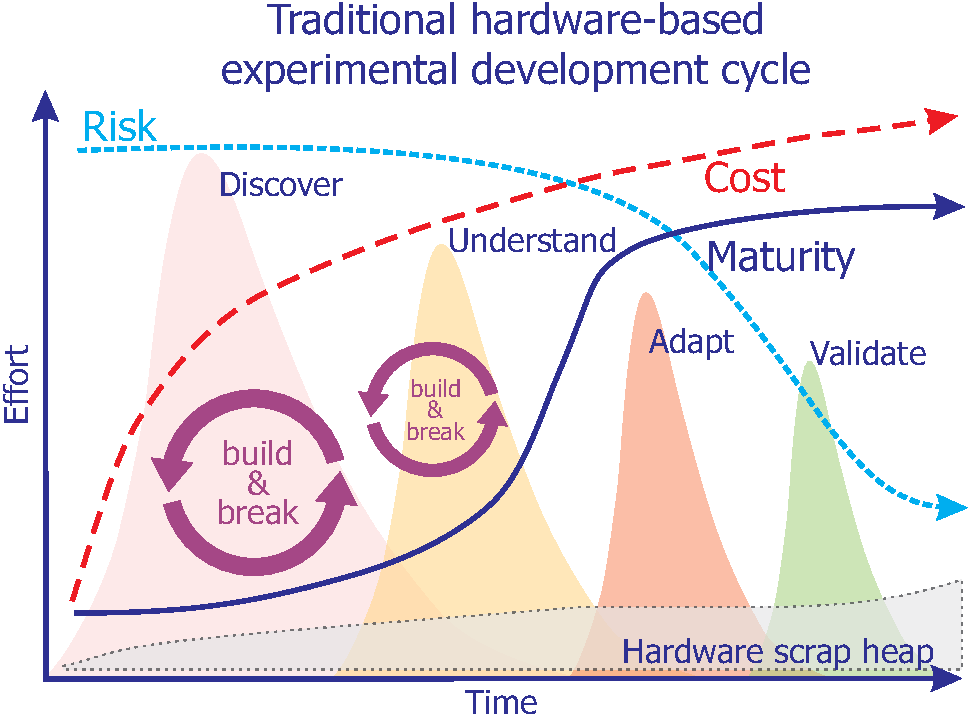
\includegraphics[width=0.46\textwidth]{pic/scesysinvest01}\hfill
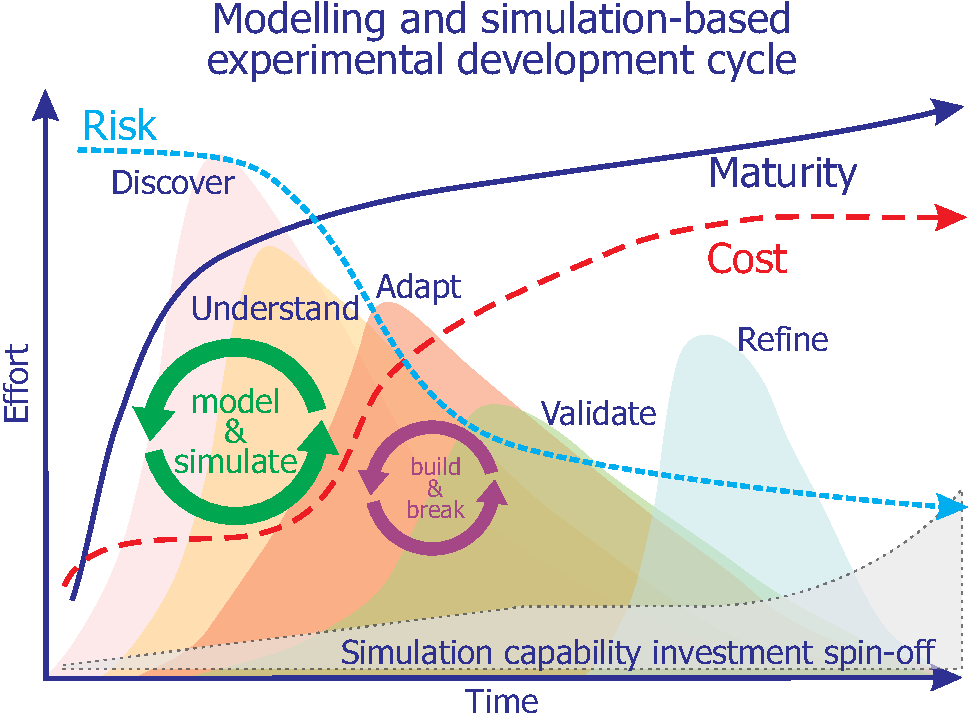
\includegraphics[width=0.46\textwidth]{pic/scesysinvest02}
\caption{Hardware-based vs simulation-based development  \label{fig:scesysinvest01}}
\end{figure}

Figure~\ref{fig:scesysinvest01}\footnote{This diagram is comprehensively adapted and expanded from a very old Airbus Industries source.  The original reference to this diagram is unfortunately lost.} shows the benefit of simulation during product development, as compared to traditional hardware build-and-break development. Key to this approach is model-based development, where equivalent models are maintained in the hardware and the simulation environment.  This approach is also sometimes called the 'Digital Twin' approach, with the 'digital' referring to the simulation model and the 'twin' referring to the equivalence between the hardware and the simulation models. Hence the terms digital twin, model-based development and simulation-based development has a strong common theme, albeit with some nuance differences.

During traditional hardware-based development, learning comes from building and  breaking hardware, in an iterating cycle. Every experiment requires a new design, build and test. This is a very time and cost intensive process, where small increments in learning comes from many hardware build cycles. 
The development phases of discovery, understanding, adaptation, and validation follow in linear sequence with little or no overlap.
Costs rise quickly and learning comes slowly. Moreover, what is learnt is not easily extended to new challenges because the experimentation did not cover the new challenges.  At the end of the project most of the funds were invested in an expensive heap of scrap metal and electronics, fit only for recycle.

Simulation-based development supports experimentation in simulation domain with much shorter cycle time and significantly lower hardware cost.  Very many experiments, many of which cannot be executed on hardware, lead to fast growth in discovery and understanding.  The development phases of discovery, understanding, adaptation, and validation now overlap significantly. Here, discovery, understanding, and adaptation are executed in very fast, as if in  single phase. Once the design is well understood the hardware experimentation commences, with much higher success rate.
While hardware development is taking place, the discovery and understanding continues and leads to product improvement that can be phased into the hardware development (typically by means of embedded software releases). 
The initial and running execution cost of simulation-based development is higher, because software models must be developed (not required for hardware-based development). However this cost is an investment, because at the end of the project a detailed functional simulation is available for use in product upgrades or for the development of new products.

The risk for hardware development remains high until validation is complete, by which time it is too late to effect major changes.  The simulation approach allows easy adaptation with continuous validation, resulting in lowering the risk from relatively early phases.  By the time the project commits to hardware builds the design is already well tested in simulation.

When comparing the two approaches' end-of-development status the hardware approach normally demonstrates increased costs and stagnation in maturity growth --- despite the increasing costs the learning has stopped. The simulation approach shows less cost increase because the risks were addressed early during development. The simulation remains a working experimental laboratory and there is continued growth in learning, even beyond the end of the development program.



\begin{figure}[tp]
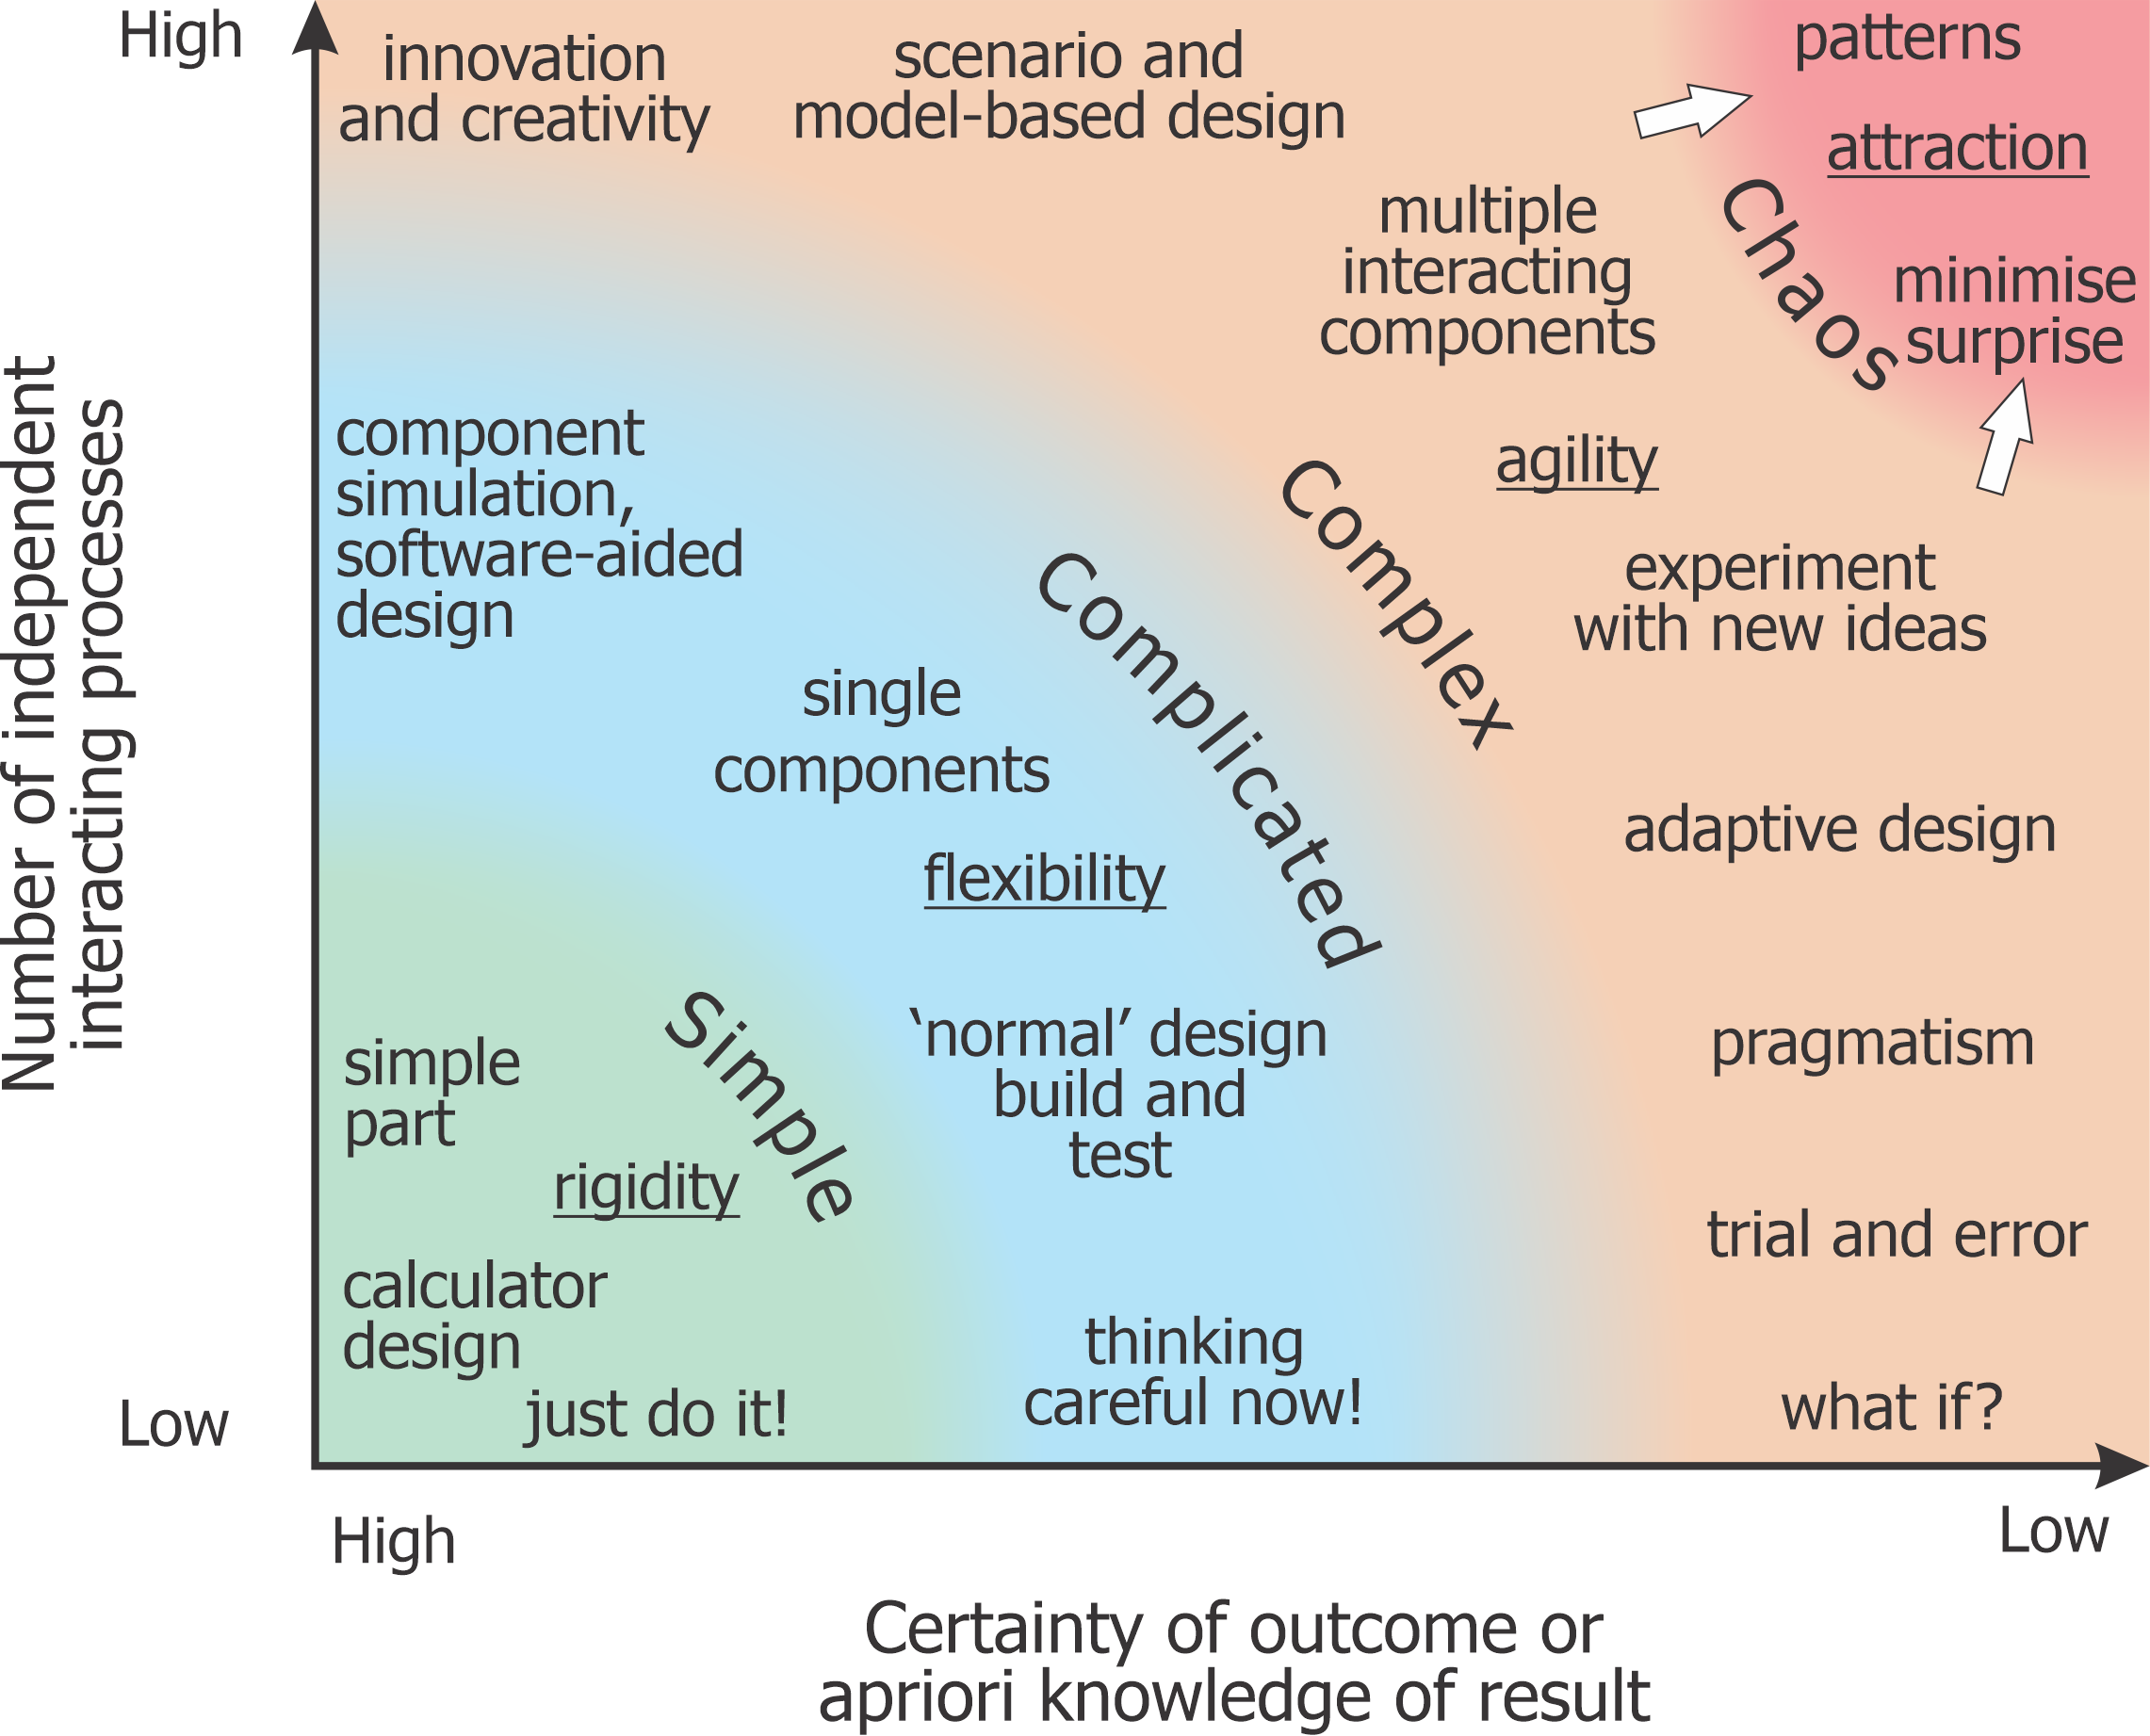
\includegraphics[width=0.7\textwidth]{pic/scesysinvest04}
\caption{Complexity and design \label{fig:scesysinvest04}}
\end{figure}

Stacey's Agreement and Certainty Matrix 
\cite{Stacey1996}
has been multiply re-interpreted in different applications, despite Stacey himself removing the diagram from his recent books \cite{Stacey2016}.  The diagram maps certainty of information on one axis against the number of degrees of freedom on the other axis. 
Figure~\ref{fig:scesysinvest04} shows our interpretation of this matrix in the context of complex weapon design.  

In the lower left (green) corner of Figure~\ref{fig:scesysinvest04} the design process is simple: certainty is high and there are few degrees of freedom. At the risk of oversimplification consider dropping a rock or a sandbag on a target: there are few free parameters most of which are relatively well understood (but not necessarily well controlled) and the physics of gravity and drag are well understood.  There is no need for a complex simulation at battle domain or theatre level.

As the systems' internal operation becomes more complex more sophisticated design tools are required (blue band). Things are complicated but not yet complex in the mathematical sense.
Consider designing a rifle: there are more free parameters, some of which are well understood (but not well necessarily controlled), and the physics of projectiles and knowledge of combustion, which are well understood. Design tools here would include \ac{CAD}, \ac{CFD} and chemical combustion models. Yet there is no need to model at theatre level.
It might be feasible to design guided munitions at this level, but the designs would probably be sub-optimal, with compromised performance.

In the (mathematically complex) brown region the systems' internal operation becomes more complex, and \textit{more interdependent on the adversary or environment}. Scenario-based design is required to model the system itself, and also the environment in which it operates, under realistic deployment conditions.
It is imperative to accurately model the adversary behaviour, and particularly details of the environment. The full representation of the system's environment must be given: the more complete, the better the evaluation.  At this level statistical aggregation (Monte Carlo runs) is required, but in the context of the full theatre. For example, the noise in a detector may minutely increase the guidance command, then the jitter on a servo may veer the missile such that the sensor observes a flash of sunlight reflection from the aircraft canopy, which just happened to be at that attitude at that moment. If the initial noise was less, none of this would have happened.  The outcome from each missile flight is different, sometimes with surprising effect. Prior missile development work shows acquisition ranges variations from  95\% of the mean to 111\% of the mean, just from random effects (noise in several components). This 15\% spread becomes important when interpreting flight test results: was the observed performance within the statistical spread?

The primary objective of any guided munition development is to maximise kill probability.  Loss of kill may be because of inherent limitations or it may result from a preventable disturbance in the flight playout.
Preventable losses can be considered to fall in the red chaos region on the top right corner in Figure~\ref{fig:scesysinvest04}.  Scenario-based simulation has been demonstrated as an effective development aid to minimise the red chaos region in a guided munition's performance.

In both the complex (brown) and chaos (red) regimes the development process requires flexible experimentation to find solutions to the tough corner case problems.  To push the limit, you have to test and evaluate on the limit, and this is only possible with a detailed scenario-based development strategy, a disciplined methodology, and suitable supporting tools.



\section{Digital Twins}
While the terminology has changed over time, the basic concept of the Digital Twin
model has remained fairly stable from its inception in 2002. It is based on the idea
that a digital informational construct about a physical system could be created as an
entity on its own. This digital information would be a ``twin'' of the information that
was embedded within the physical system itself and be linked with that physical
system through the entire lifecycle of the system \cite{Grieves2017}.

The digital twin concept is very strong in manufacturing and maintenance using networked sensors (\ac{IoT}) to monitor deviations in  hardware performance relative to the \textit{reference model} which is the ideal design as captured in a model or digital form \cite{Tao2017-0233-1}.  If the deviations are sufficiently large, maintenance is indicated.


\begin{figure}[tp]
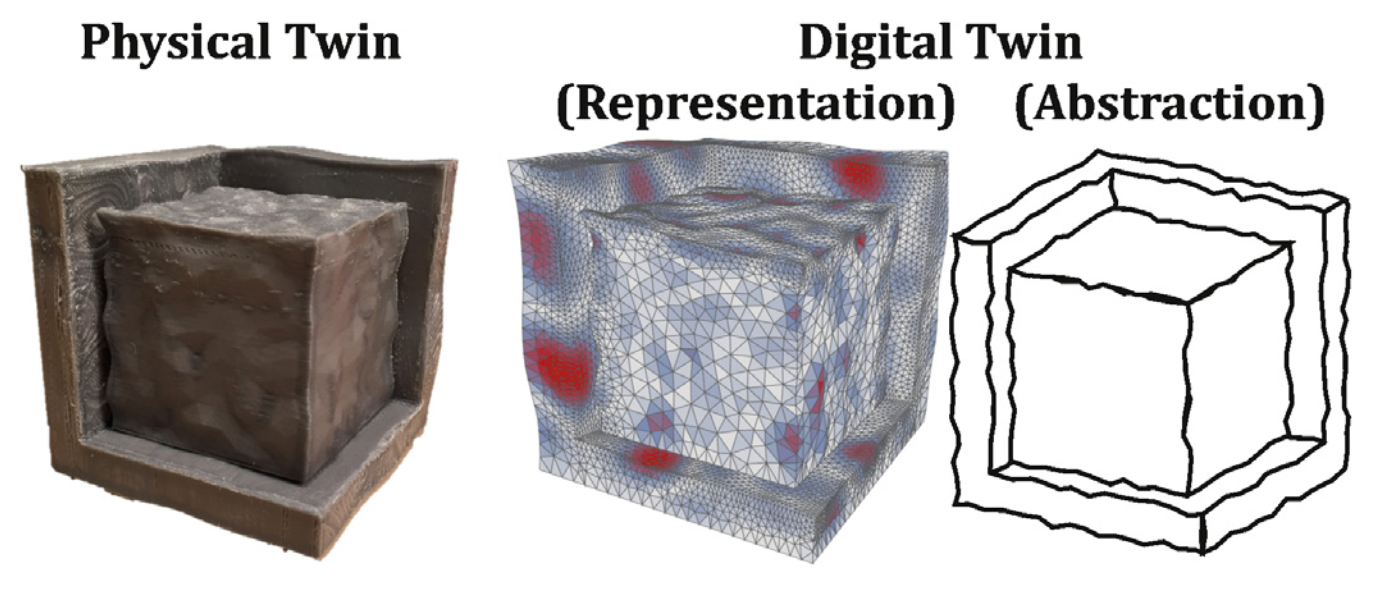
\includegraphics[width=0.55\textwidth]{pic/digitaltwin01}
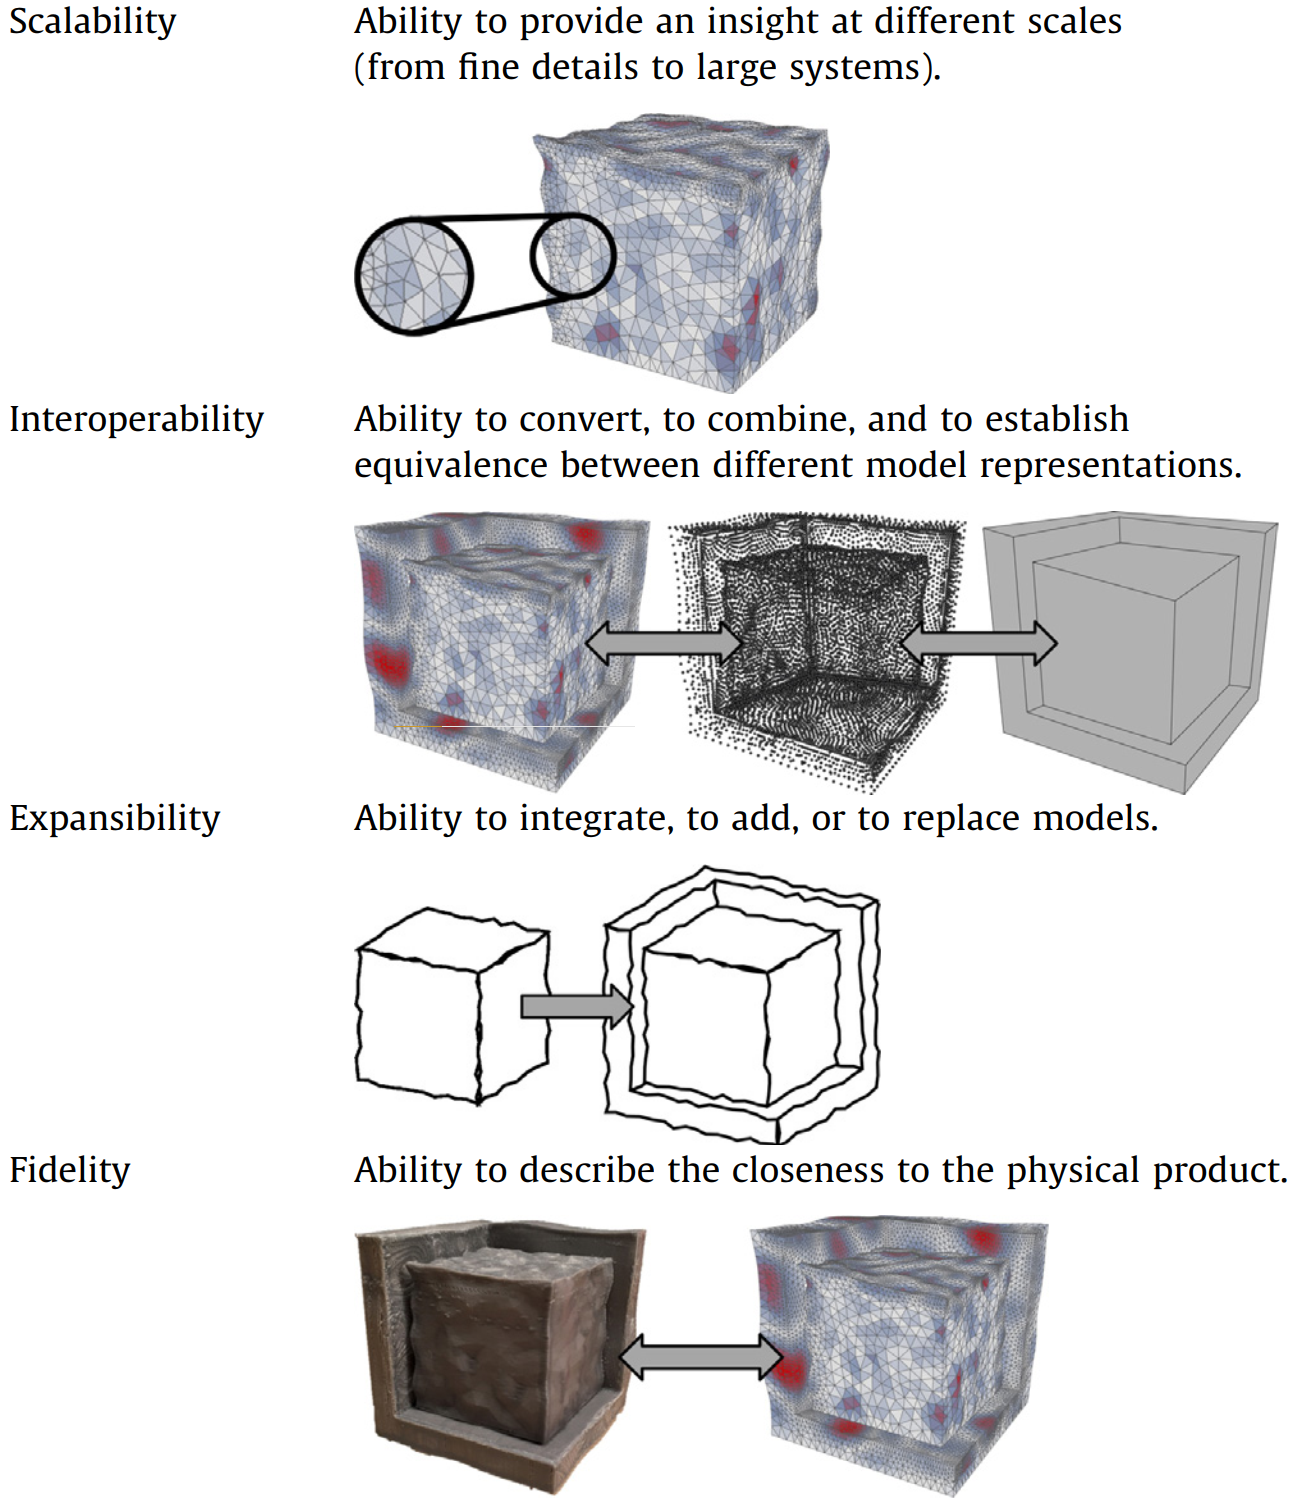
\includegraphics[width=0.7\textwidth]{pic/digitaltwin02}
\caption{Requirements for digital twins \cite{Schleich-2017}\label{fig:digitaltwin01}}
\end{figure}

Although this is not how we see the digital twin during development, see Zweber's definition \cite{Zweber2017}, quoting the `Glossary of Defense Acquisition Acronyms and Terms', defines the digital twin as: ``The \ac{DTw} is an integrated multiphysics, multiscale, probabilistic simulation of an as-built system, enabled by Digital Thread, that uses the best available models, sensor information, and input data to mirror and predict activities/performance over the life of its corresponding physical twin.  Only after the physical configuration of the system is sufficiently defined in the detailed design phase, will the DTw be meaningful. The DTw comes into existence when
the system development lifecycle reaches the bottom of the V-diagram.'' See Zweber's paper \cite{Zweber2017} for more detail on how they see the bigger picture of Digital Engineering as part of systems engineering, of which the digital twin is only a part.  He does elaborate on the role of a digital twin during development. 

Schleich \cite{Schleich-2017} considers digital twins in design and production engineering. He provides a nice pictorial representation of the main requirements of a digital twin (Figure~\ref{fig:digitaltwin01}).  He quotes \cite{Boschert2016} in his definition of a digital twin: ``the vision of the digital twin itself refers to a comprehensive physical and functional description of a component, product or system, which includes more or less all information which could be useful in all --- the current and subsequent --- lifecycle phases.''
The requirements shown in Figure~\ref{fig:digitaltwin01} also apply accurately to the model-based approach advocated in this chapter.  He makes an important statement: 
``there is a strong need to integrate all life-cycle data artefacts into a comprehensive management system, which can be used by various actors for querying data, such as through-life performance
information, and making predictions about the physical product from the digital twin for design optimization and manufacturing system improvement.''  


Boschert \cite{Boschert2016} states the following requirements for digital twins in simulation:
``The Digital Twin refers to a description of a component, product or system by a set of well aligned executable models with the following characteristics:
\begin{enumerate}
\item The Digital Twin is the linked collection of the relevant digital artefacts including engineering data, operation data and behaviour descriptions via several simulation models.  The simulation models making-up the Digital Twin are specific for their intended use and apply the suitable fidelity for the problem to be solved.

\item The Digital Twin evolves along with the real system along the whole life cycle and integrates the currently available knowledge about it.

\item  The Digital Twin is not only used to describe the behaviour but \textit{also to derive solutions relevant for the real system, i.e. it provides functionalities for assist systems to optimize operation and service}. Thus, the Digital Twin extends the concept of \ac{MBSE} from engineering and manufacturing to the operation and service phases.''
\end{enumerate}


% \begin{figure}[tp]
% \includegraphics[width=0.7\textwidth]{pic/scesysinvest09.pdf}
% \caption{The five dimensions of digital twins, derived from \cite{MengZhang2020}\label{fig:scesysinvest09.pdf4}}
% \end{figure}

Zhang \cite{MengZhang2020} defines five dimensions relevant to digital twins (Figure~\ref{fig:scesysinvest09.pdf4}): (1) the physical entity, (2) the virtual entity, (3) the data, (4) services to support the twin, and (5) communication connections between all of these.  The importance of this  view is that services, data and communication between these parts are as much part of the digital twin as the physical entity.  For example, if a system requires geographic data from Google Earth or some observation platform, this service is an integral part of the twin concept. Likewise, the data in the twin concept is incredibly important and must be conserved and managed as for the physical entity. Finally, Zhang's model shows that there is a constant iterative interaction between all the parts: without the interaction (e.g., design revision), the digital twin concept is static, missing out on opportunities for growth.

The original definition, shown on the left in Figure~\ref{fig:scesysinvest09.pdf4} extends on the common view of the digital twin as physical and virtual entities, but still retains the concept as for a single object (e.g., a vehicle, spaceship, etc.). We extend the notion by considering \textbf{the system as a collection of digital twins}: for example a missile comprises a sensor, gimbal, signal processing, airframe and guidance, etc. In the context of a development simulation system, each of the components are managed as separate digital twins. For example, the sensor design team maintains their own set of physical hardware, virtual models, data sets, etc.  The sensor design process iterates internally in the optimisation of the sensor design.  However, the individual components also interact with each other to build up the system.

Our past experience with scenario- and model-based missile design is that the component-level design optimisation iterations take place inside the design teams, where the hardware designers and simulation modelling experts maintain the \textbf{model-based design} of their component.  The system-level interaction brings together all the components and this is where the system designer/engineer uses  \textbf{scenario-based design} to evaluate and optimise system performance.

\begin{figure}[tp]
\centering
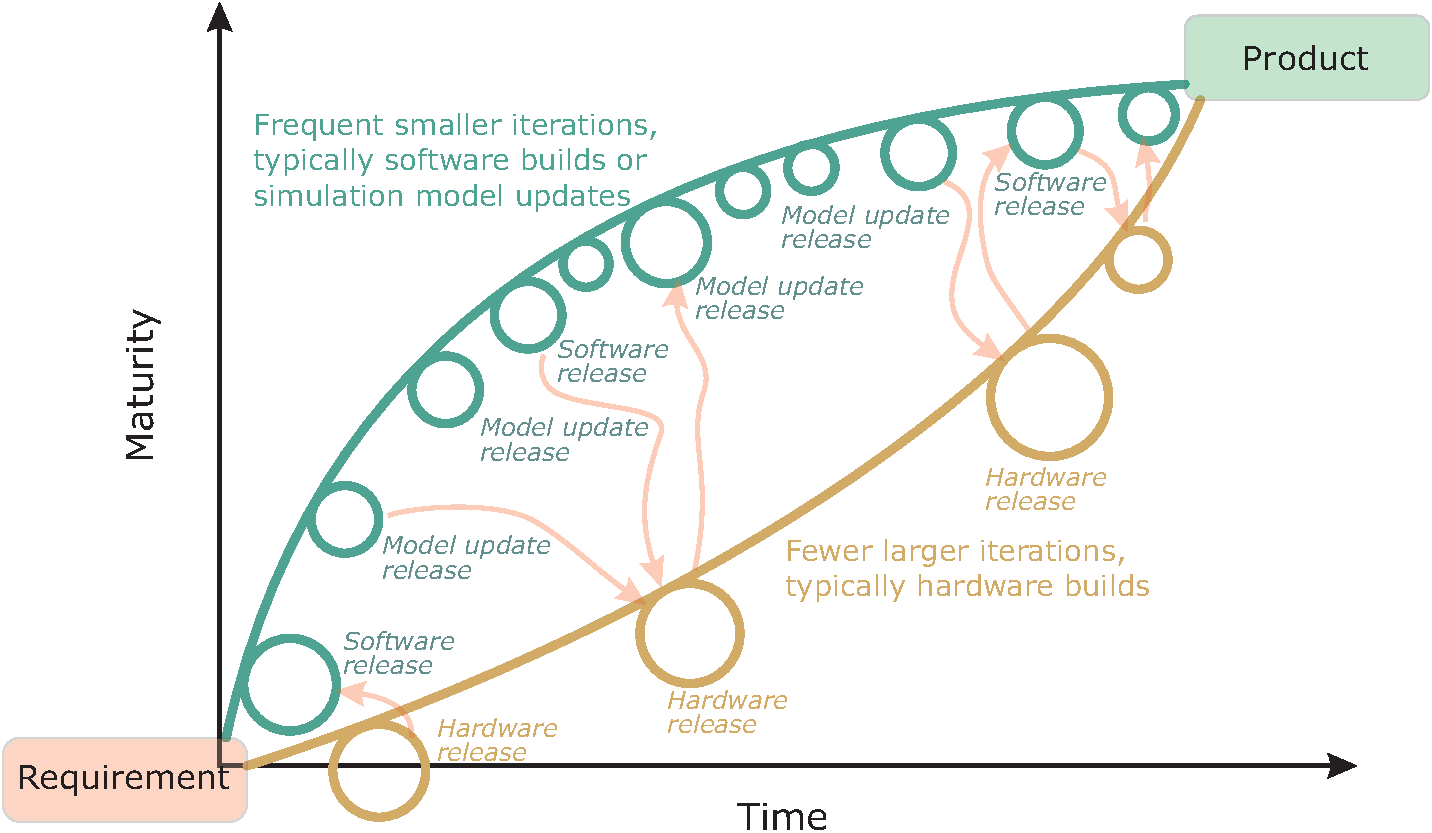
\includegraphics[width=0.8\textwidth]{pic/scesysinvest07}
\caption{Integrated iterative development\label{fig:scesysinvest07}}
\end{figure}

Some  design cycles iterates at very short intervals (e.g., software algorithms), whereas other design cycles are slower (hardware designs), see Figure~\ref{fig:scesysinvest07}. The iterated short-cycle sequence leads to quicker growth in maturity; this is particularly useful in complicated designs such as software algorithms.
The model-based simulation provides an arena where design sequences with different iteration cycle periods can be effectively integrated. There is no need to keep all design processes on the same time sequences. The simulation can use the latest versions of all available components. Good order requires careful configuration control, but this is relatively easily done with modern software tools and disciplined system engineering practices.

% \begin{figure}[tp]
% \includegraphics[width=\textwidth]{pic/tao-DT-design-cycle.png}
% \caption{Digital twin design improvement cycle \cite{Tao2018-1443229} \label{fig:tao-DT-design-cycle.png}}
% \end{figure}

Tao \cite{Tao2018-1443229} describes a digital twin-driven product design framework as summarised in Figure~\ref{fig:tao-DT-design-cycle.png}.  The example describes the fast-cycle iterative improvement of a bicycle design.  The key principle here is that the bicycle design and manufacturing process are verified on the model before committing to hardware manufacture.  Note also, that once the model is available all future upgrades only require small modifications of the existing model.  The product-improvement cost therefore decreases in future generations. 

